\documentclass[10pt]{article}
\usepackage[polish]{babel}
\usepackage[utf8]{inputenc}
\usepackage[T1]{fontenc}
\usepackage{graphicx}
\usepackage[export]{adjustbox}
\graphicspath{ {./images/} }
\usepackage{amsmath}
\usepackage{amsfonts}
\usepackage{amssymb}
\usepackage[version=4]{mhchem}
\usepackage{stmaryrd}

\title{Zestaw 11 }

\author{}
\date{}


\newcommand\Varangle{\mathop{{<\!\!\!\!\!\text{\small)}}\:}\nolimits}

\begin{document}
\maketitle
\begin{center}

\includegraphics[max width=\textwidth]{2024_11_21_6b9e619025c2bae5b52ag-1(1)}
\end{center}

\section*{GIMNAZJUM}
\begin{enumerate}
  \item Punkt \(M\) jest środkiem boku \(A B\) trójkąta \(A B C\). Na środkowej \(C M\) znajduje się taki punkt \(D\), że \(A C=B D\). Udowodnij, że \(\Varangle M C A=\Varangle M D B\).
  \item Czy istnieje taka całkowita dodatnia liczba \(n\), że \(2 n\) jest kwadratem liczby\\
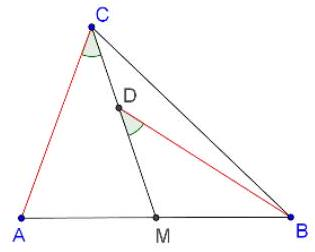
\includegraphics[max width=\textwidth, center]{2024_11_21_6b9e619025c2bae5b52ag-1}\\
całkowitej, zaś 1024n jest czwartą potęgą liczby całkowitej? Odpowiedź uzasadnij.
  \item Pan Kowalski sprzedaje buty. Dziś rano przyszedł do niego klient i dość szybko zdecydował się na mokasyny za 80 zł. Wręczył panu Kowalskiemu banknot 200 zł, ale ten niestety nie miał wydać. Poszedł więc do sąsiedniego kiosku i rozmienił 200 zł. Klient zabrał buty i 120 zł reszty i poszedł. Po dziesięciu minutach do sklepu pana Kowalskiego wpadł zdenerwowany właściciel kiosku stwierdzając, że wręczony mu banknot 200 zł jest fałszywy. Niestety, klient dawno zniknął i pan Kowalski musiał oddać 200 zł z własnych pieniędzy. Pan Kowalski był smutny - dzień się tak dobrze zapowiadał, a on tyle stracił. No właśnie - ile stracił? Przyjmujemy, że buty były warte 80 zł.
\end{enumerate}

\section*{LICEUM}
\begin{enumerate}
  \item Czy istnieją takie cztery dodatnie liczby całkowite, że dowolne dwie z nich mają największy wspólny dzielnik większy od 1, a dowolne trzy z nich mają największy wspólny dzielnik równy 1? Odpowiedź uzasadnij
  \item Rozwiąż układ równań
\end{enumerate}

\[
\left\{\begin{array}{c}
x^{2}=y+z \\
y^{2}=z+x \\
z^{2}=x^{2}+y^{2}
\end{array}\right.
\]

\begin{enumerate}
  \setcounter{enumi}{2}
  \item Jakie są dwie ostatnie cyfry liczby \(2011^{2011}\). Odpowiedź uzasadnij.
\end{enumerate}

Rozwiązania należy oddać do piątku 17 kwietnia do godziny 12.30 koordynatorowi konkursu panu Jarosławowi Szczepaniakowi lub swojemu nauczycielowi matematyki.

Na stronie internetowej szkoły w zakładce Konkursy i olimpiady można znaleźć wyniki dotychczasowych rund i rozwiązania zadań.


\end{document}